\subsection{Data and split}
The supplied competition data contain 707 physical training disks and 180 unlabeled test disks. Images are grayscale, 8-bit JPEGs at \(2048\times2048\) pixels. The training JSON contains 1,154 independent annotator views and 8,199 nonempty filament annotations. Multiple views of a JPEG share one physical image ID; an annotator prefix identifies the view. We decode each polygon into a native binary mask with COCO utilities. We use no external labels, observations, weights or inference inputs.

We place physical images in 27-day UTC blocks and reserve Udaipur as the site transfer test. A 48-hour temporal embargo removes cross-fold neighbors. The final split contains 336 training, 115 development, 80 confirmation, 101 site-transfer and 75 purged disks. The closest retained cross-fold pair is 48 hours and 20 seconds apart. An independent audit found no repeated JPEG bytes or high-correlation pairs in a low-resolution image screen. This reduces the risk of nearly repeated images crossing the split; it does not prove that long-lived features never recur.

\subsection{Image representation and model}
For each disk, we sample pixels from the central square and subtract its median. We divide by the 90th-to-10th percentile range with a 16-gray-level floor and clip to \([-4,4]\). This retains local dark contrast while limiting the effect of exposure differences. Development annotations show median skeleton width of approximately 8.3 native pixels, so we retain native pixels in the network and export.

Our compact U-Net \cite{ronneberger2015unet} uses five encoder levels, four decoder stages, two \(3\times3\) convolutions per block, group normalization and SiLU activations. Base width is 24 and doubles on each downsampling step; the model has 4.37 million parameters. Transposed convolutions upsample the decoder, which receives encoder features at each scale through skip connections. The final \(1\times1\) convolution predicts a foreground logit.

For each annotation view we take the union of its filament masks. The mean of these unions across views gives a soft training label, so ambiguous pixels need not be forced to a binary consensus. We sample five \(384\times384\) crops per physical observation per epoch. With probability 0.65 we anchor a crop near an annotated bounding box, with bounded jitter; otherwise we sample uniformly. We apply right-angle rotations, a random reflection and modest intensity scaling and shifts. The training objective is pixel-weighted binary cross entropy plus soft Dice loss. AdamW starts at \(7\times10^{-4}\) and uses a cosine schedule. We train from random initialization, with batch size 12 and seed 271828, on an RTX 4090.

\subsection{Native inference and instance extraction}
We tile the normalized \(2048\times2048\) disk at stride 288 with the last tile aligned to each edge. We accumulate sigmoid probabilities with taper weights near overlap boundaries and divide by the total weight at each pixel. The reconstructed probability map is stored as float16 before instance extraction. An independent pointwise fixture checked every reconstructed pixel and found a maximum error of \(2.44\times10^{-4}\) after float16 rounding. This checks tile placement; a four-disk development check reproduced the chosen stride exactly but changing it to 256 shifted foreground IoU to 0.876--0.922. We therefore lock the tiling grid for reproduction.

We threshold the native map, use eight-neighbor connected components and drop regions smaller than a calibrated area. A fixed 24-image development subset selects epoch 24. We then recalibrate on all 115 development maps and freeze a probability threshold of 0.65 and minimum area of 700 native pixels. Confirmation and site-transfer observations play no role in either decision. Each output instance is one native compressed COCO RLE. Its row ID combines the unchanged observation stem and a unique suffix. For images with zero predicted instances, the export emits no placeholder row, and the coverage record still accounts for the image.

\begin{figure*}[t]
\centering
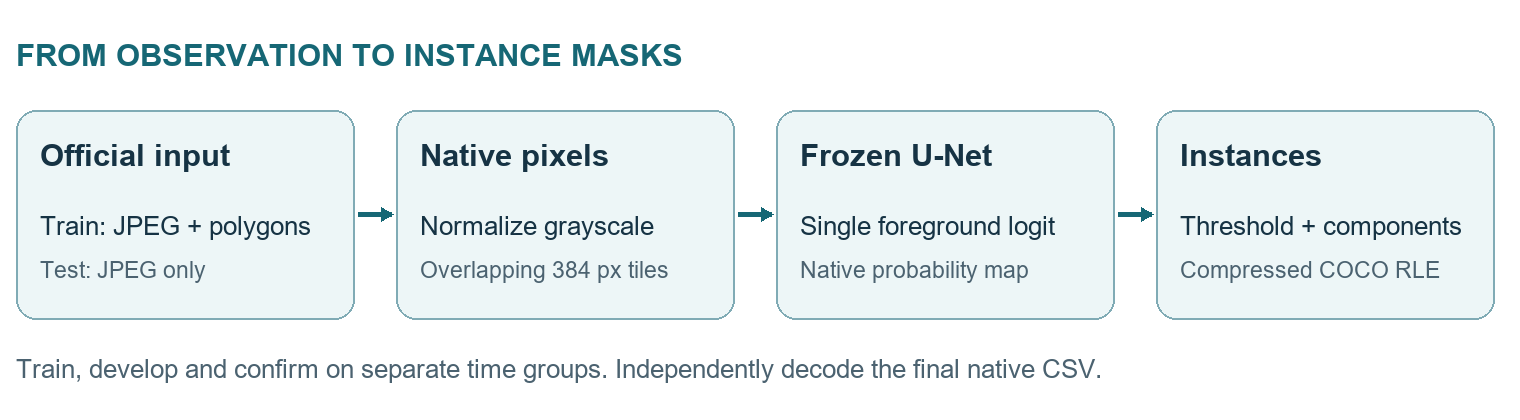
\includegraphics[width=\textwidth]{pipeline.png}
\caption{Training and inference paths. Test inference uses the supplied H-\(\alpha\) JPEG and the frozen model.}
\end{figure*}

\subsection{Challenger: disk-aware local contrast}
We considered short-gap repair because GONG seeing and opacity variation can interrupt an otherwise coherent filament. The development audit found 298 predictions with zero overlap with the corresponding annotation view: 101 in the disk interior, 189 at projected radius \(0.8\) to \(0.95\,R\), two near the rim and six off disk. It found 73 meaningful splits but only six with a short, directionally supported gap. Only one of those had a fragment pair whose truth-informed union would recover a missed match. We therefore tested local contrast as the single challenger.

For each disk we fit a circle to outward intensity drops along 180 radial rays. For each baseline instance we skeletonize the component, estimate width from its interior distance transform and sample an adjacent flank band. Flank pixels must lie within \(0.98\,R\) and outside any predicted foreground. With flank median \(m_f\), skeleton median \(m_s\) and flank median absolute deviation \(d_f\), the score is
\[
 c=\frac{m_f-m_s}{\max(2,\ 1.4826d_f)}.
\]
A component is retained unchanged if its score meets the contrast floor. We retain the baseline instance when the disk fit or local background is unreliable. The challenger changes neither network probabilities nor accepted mask boundaries. The floor is selected on development groups, keeping all other settings and inputs fixed.

H-\(\alpha\) contrast is an observed intensity difference, not evidence of magnetic connectivity. Dark active-region structures can pass the filter, and genuine faint structures can fail it. GONG display JPEGs already suppress large-scale intensity variation; we use local flanks rather than fitting a global limb-darkening correction.

